\documentclass[a4paper,12pt]{article}
\usepackage[utf8]{inputenc}
\usepackage{xcolor}
\usepackage{url}
\usepackage[T2A]{fontenc}
\usepackage{graphicx}
\usepackage[margin=80pt]{geometry}
\usepackage{booktabs}
\usepackage{natbib}

\usepackage[english,serbian]{babel}

\begin{document}

\title{\textbf{Žene u programiranju\\} \small{Seminarski rad u okviru kursa\\Tehničko i naučno pisanje\\ Matematički fakultet}}

\author{Jelena Veličković\\ mi21203@alas.matf.bg.ac.rs \and Bojana Zagorac\\ mi22135@alas.matf.bg.ac.rs \and Miloš Bigović\\ mi22149@alas.matf.bg.ac.rs \and Zorana Jevtić\\ mi22148@alas.matf.bg.ac.rs}

\date{\textit{\center{Novembar, 2022.}}}

\maketitle

\begin{abstract}
    U ovom tekstu je ukratko objašnjen doprinos žena u programiranju uz priloge. Takođe, biće reči o
    brojnosti žena koje se time bave, kao i o Adi Bajron, najistaknutijom ženom programerom. Suština 
    ovog teksta je razbijanje predrasude da se programiranjem bave isključivo muškarci, odnosno da je 
    programiranje "muški posao". 
\end{abstract}


\color{blue}\tableofcontents

\newpage
\color{black}\section{Uvod}
\begin{flushleft}
Odgovor na pitanje da li se programiranjem česce bave žene ili muškarci, u većini slučajeva bi bio muškarci. Pitali smo se zašto je to tako i u svom radu smo ukazali na greske koje dovode do ovog stereotipa. 
Iako se danas programiranjem češće bave muškarci, iznenadiće vas sam početak razvijanja informatičke industrije. 

U radu predstavljamo početke informatike i same inicijatore ove tada nove i neistražene sfere. Znamo da ni danas u potpunosti informatika nije istražena, ali kako je sve pocelo i kako su se tada ljudi izborili sa novinama, pokusali smo da predočimo na najbolji mogići način kroz same primere. U samom radu mozemo videti koliko je informatika zapravo napredna i kojom se brzinom razvija, da li je to zbog broja ljudi koji svakodnevno rade na projektima, ili je informatici u samoj prirodi da se razvija i širi.
\end{flushleft}

\section{Ada Bajron}

\begin{flushleft}
    Ejda Bajron(1815-1852.), poznata kao Ada, smatra se prvim programerom zbog svog programa, kojim se pomocu analitičke mašine izračunavaju Bernulijevi brojevi. Odnosno, učestvovala je u realizaciji projekta analitičke mašine finansijski i svojim idejama. Njena najznačajnija ideja u realizaciji tog projekta je bio prenos kontrole i rad sa ciklusima. Iako se primarno bavila matematikom, to nije značilo da se tu zaustavljaju njena interesovanja. Za razliku od mnogih u to doba, bila je inovativna smatrajući da se analitička mašina može upotrebljavati za opštije stvari, kao i u naučne svrhe. To je u budućnosti i realizovano, dakle savremeni računari se upravo uklapaju u tu njenu zamisao. Upoznavši poznatog matematičara Čarlsa Bebidža, nakon nekog vremena mu se pridružila u projektu kao njegov tumač. To jest, jasno je opisala kako će mašina funkcionisati, čime je doprinela računarskoj nauci. Objasnila je da je suština rada analitičke mašine tkanje algebarskih obrazaca poput Žakardove mašine koja je radila po principu kreiranja slika na osnovu bušenih kartica. Predmet svojih proučavanja i rada je nazivala naukom i operacijama, međutim to je zapravo računarstvo. Nije ni čudno to što je razmišljala na tako genijalan način, s obzirom na to da je spojila maštovitost sa racionalnošću. Umetničku crtu je nasledila od oca lorda Bajrona, romantičarskog pesnika, dok je zahvaljujući majčinom uticaju uspela da stvori ravnotežu i izbegne površan pristup. Bez obzira na to što su neki naučnici pokušavali da ospore njen rad i doprinos, mnogi su odbacivali ovo tumačenje. Razlog osporavanja je bio čuvanje moći u rukama mučkarca kao i predrasude prema ženama koje se bave programiranjem zbog spoznaje važnosti i značaja te naučne oblasti. Vrhunac njene karijere je programski jezik nazvan Ada u njenu čast, kao i priznanje koje dobija svake godine 15. oktobra, počevši od 2009. godine, kako bi se istakao naučni rad i doprinos žena koji je zanemaren i nipodaštavan. Na slici 1, prikazana je Ada Bajron.
\end{flushleft}

\begin{figure}[h]
    \centering
    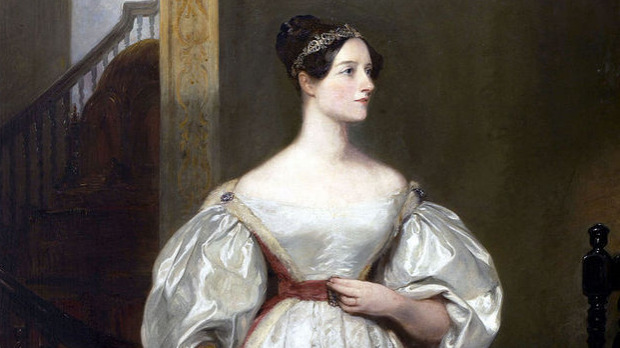
\includegraphics[width = .6\textwidth]{adabajron.jpg}
    \caption{Ada Bajron}
    \label{fig:my_label}
\end{figure}


\newpage
\section{Margaret Hamilton}

\begin{flushleft}
 Margaret Hamilton (rođena 17. avgusta 1936, Paoli, Indijana, SAD), američki informatičar koja je bila jedan od prvih programera kompjuterskog softvera, stvorila je termin softverski inženjer da opiše svoj rad. Pomogla je u pisanju kompjuterskog koda za komandne i lunarne module korišćene u misijama Apolo na Mesec kasnih 1960-ih i ranih 70-ih.

    Studirala je matematiku i filozofiju na Earlham koledžu u Ričmondu, Indijana. Nakon diplomiranja 1958. godine kratko je predavala matematiku u srednjoj školi. Iako je Margaret planirala da studira apstraktnu matematiku na Univerzitetu Brandeis, prihvatila je posao na Tehnološkom institutu u Masačusetsu (MIT) dok je njen suprug pohađao Pravni fakultet Harvarda. Na MIT-u je počela da programira softver za predviđanje vremena i radila je na postdiplomskim studijama iz meteorologije.
    Početkom 1960-ih Hamiltonova se pridružila MIT-ovoj Lincoln laboratoriji, gde je bila uključena u projekat Poluautomatsko zemaljsko okruženje (engl.Semi-Automatic Ground Environment, SAGE), prvi američki sistem protivvazdušne odbrane. Posebno je napisala softver za program za otkrivanje neprijateljskih aviona. Hamilton je zatim radila u kompaniji "MIT’s Instrumentation Laboratory" (sada nezavisna laboratorija Charles Stark Draper), koja je obezbedila aeronautičku tehnologiju za Nacionalnu upravu za aeronautiku i svemir (NASA). Predvodila je tim koji je imao zadatak da razvije softver za sisteme navođenja i kontrole komandnih i lunarnih modula misija "Apolo" u letu. U to vreme nijedna škola nije predavala softversko inženjerstvo, tako da su članovi tima morali sami da rešavaju probleme. Ona je kreirala termin softverski inženjer jer je smatrala da je posao koji ona i njen tim obavljaju jednako važan i jednako inženjerski kao i drugi rad na svemirskoj letelici Apolo. Sama Margaret se posebno koncentrisala na softver za otkrivanje sistemskih grešaka i za oporavak informacija u slučaju pada računara. Oba ta elementa bila su presudna tokom misije Apolo 11 (1969), koja je odvela astronaute Nila Armstronga i Baza Oldrina na Mesec. Hamilton je napustila MIT sredinom 1970-ih da bi radila u privatnom sektoru. Bila je jedna od osnivača kompanije Higher Order Software 1976. godine. Kompanija se bavila objedinjenom metodologijom sistemskog inženjeringa koja uključuje osnovni skup principa i standardni skup alata i tehnika za razvoj računarskih sistema. Ovi principi  obuhvataju sve faze razvoja sistema i sve discipline uključujući dizajn, verifikaciju, dokumentaciju, upravljanje i održavanje. Automatizovani alati služe da eliminišu mnoge moguće izvore ljudske greške u tranziciji razvoja sistema od koncepta do primene. Osnovala je Hamilton Technologies 10 godina kasnije koja je obezbedila proizvode i usluge za modernizaciju procesa planiranja, sistemskog inženjeringa i razvoja softvera kako bi se maksimizirala pouzdanost, niži troškovi i ubrzalo vreme izlaska na tržište.

    Hamilton je bila dobitnica raznih počasti, uključujući NASA-inu nagradu o izuzetnom dostignuću.
    \end{flushleft}
    \begin{figure}[h]
    \centering
    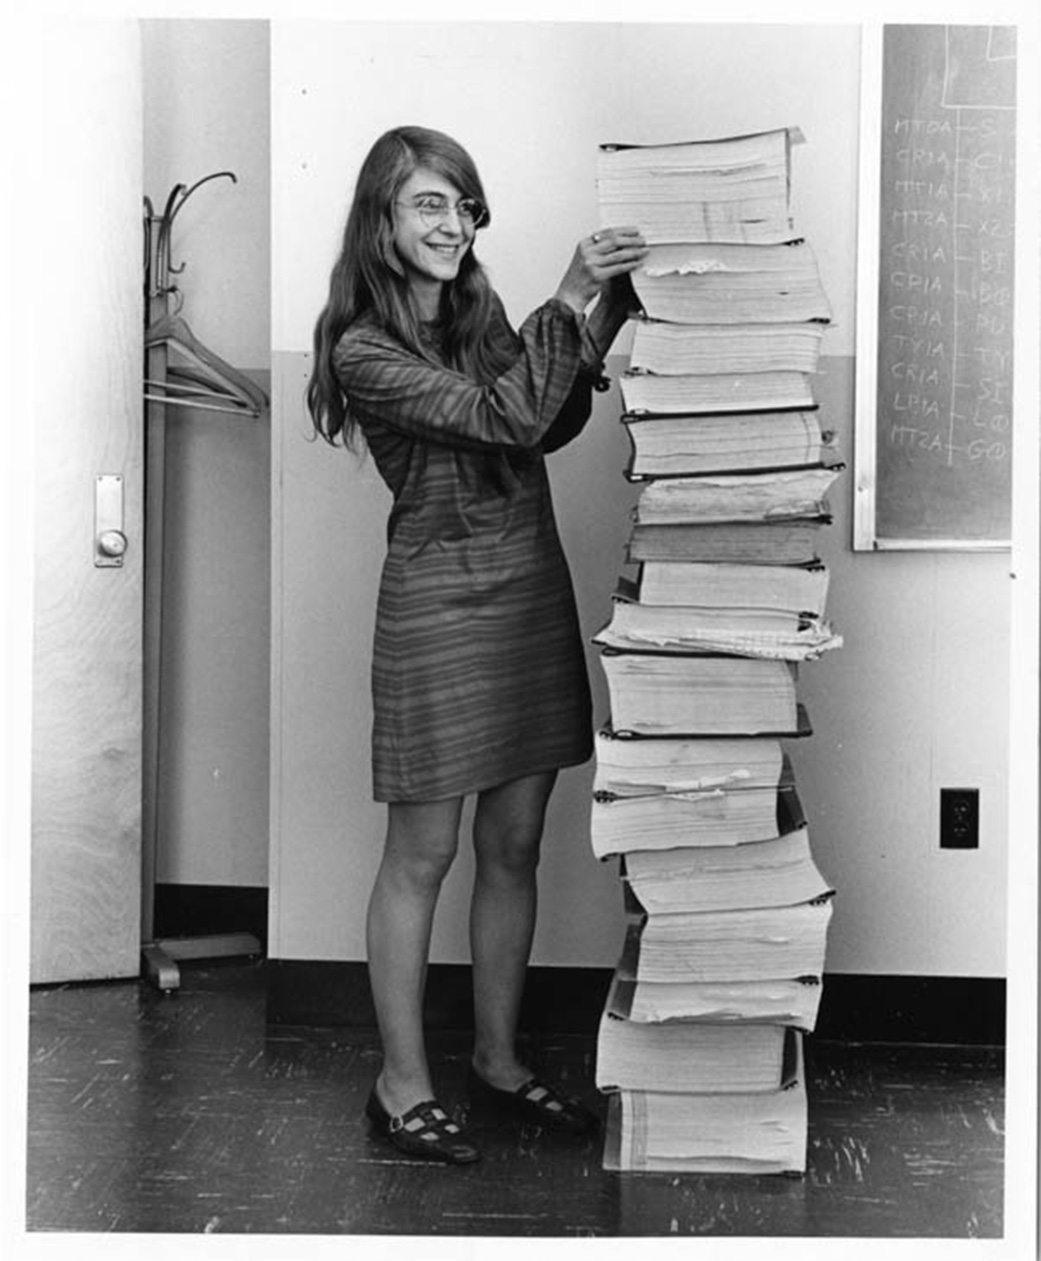
\includegraphics[width = .4\textwidth]{margaret_hamilton5.jpg}
    \caption{Margaret Hamilton}
    \label{fig:my_label}
\end{figure}

\newpage
\section{ENIAC Programeri}

\subsection{Šta je zapravo ENIAC}
\begin{flushleft}

U periodu između 1943. i 1946. godine od strane američke vojske i tima univerziteta u Pensilvaniji koji su predvodili Džon Mokli i Džej Ekert konstruisan je prvi elektronski računar opšte primene - ENIAC. Osnovna svrha bila mu je jedna specijalna namena - izračunavanje trajektorije projektila. Bilo je moguće da se mašina programira i za druge zadatke ali to je zahtevalo intervencije sa preklopnicicma i kablovima koje su mogle da traju danima. Na programiranju samog računara radilo je šest žena - Ketlin Antoneli, Rut Teitelbaum, Franses Spens, Žan Bartik, Marlin Melcer, Beti Holberton.

\end{flushleft}

\subsection{Ketlin Antoneli}
\begin{flushleft}

Ketlin Antoneli(1921-2006), poreklom iz Irske, je bila Američki programer. Svoje školovanje je započela 1927. godine u Katoličkim školama u Sjedinjenim Državama. Zatim je pohađala Katoličku srednju školu za devojke Džona V. Halahana. 1938. godine se upisala na Čestnat koledž u Filadelfiji, kojeg je i zavrsila 1942. godine.

\end{flushleft}

\subsection{Rut Teitelbaum}
\begin{flushleft}

Rut Teitelbaum(1924-1986), rođena u Njujorku, je bila jedna od prvih programera na svetu. Pohađala je Hanter koledž i zavrsila je sa bachelor degree iz matematike.

\end{flushleft}

\subsection{Franses Spens}
\begin{flushleft}

Franses Spens(1922-2012) je završila srednju školu za devojčice u Južnoj Filadelfiji 1938. godine i upisala Templ Univeritet. Ali ubrzo je dobila stipendiju Čestnat Koledža, gde je upoznala Ketlin Antoneli. Tokom studija se zaposlila kao profesor matematike u srednjoj školi. Ona je htela da bude profesorka matematike, ali 1942. godine odmah nakon zavrsenih studija je zapošljena od strane vojske.

\end{flushleft}

\subsection{Žan Bartik}
\begin{flushleft}

Žan Bartik(1924-2011), usled velikih novčanih problema, je završila Stenberi srednju školu, nakon čega je upisala Učiteljski Koledž na severozapadnom delu Misurija. Upisala je koledž sa namerom da se opredili za novinarstvo, medjutim opredelila se ipak za matematiku. Nakon završetka studija, aplicirala je za posao u IMB kompaniji i na koledžu u Filadelfiji. IBM ju je odbio ali ne i koledž, tako se prvi put susrela sa ENIAC mašinom. 

\end{flushleft}

\subsection{Marlin Melcer}
\begin{flushleft}

Marlin Melcer(1922-2008), poreklom iz filadelfije, je zavrišila Templ Univeritet u Filadelfiji 1942. godine. Zaposlila ju je vojska u Mur školi elektrotehnike na Univerzitetu u Filadelfiji, a ubrzo se učlanila u ekipu koja je radila na mašini ENIAC. 

\end{flushleft}

\subsection{Beti Holberton}
\begin{flushleft}

Beti Holberton(1917-2001) je studirala 40-ih godina proslog veka novinarstvo na Filadelfijskom Univerzitetu, što joj je omogućilo da puno proputuje. Međutim kako je krenuo rat, tako su muškarci išli u rat, a žene su bile zapošljavane za izračunavanje trajektorije samih projektila.

\end{flushleft}


\section{Zbog čega ima manje žena u IT sektoru?}

\subsection{Statistika}
\begin{flushleft}
U poslednjih 20 godina, u SAD-u ali i kod nas, je zabeležen nagli pad broja žena koje stiču fakultetske diplome iz računarskih nauka i
informacionih tehnologija. Prema Nacionalnom centru za statistiku obrazovanja, iako žene čine većinu diplomiranih fakulteta, 
one su stekle samo 19\% diploma iz informatike koje su dodeljene 2016.

Međutim, žene nisu uvek bile toliko nedovoljno zastupljene u IT sektoru. Posle Drugog svetskog rata, 
tokom digitalne revolucije (1950-1970) kompjutersko programiranje je postalo popularnije među oba pola. 
Do sredine 1980-ih godina procenat žena na kompjuterskim naukama rastao je veoma brzo i pretekao čak i rast u medicini, 
a onda kada su žene počele da u ovoj oblasti čine više od 35\% studenata, procenat je počeo naglo da pada sve do danas. 
\end{flushleft}


\begin{table}[h]
\centering
\begin{tabular}{c|c}
\toprule
Godina    & procenat zena u IT-u \\ 
\midrule
1984      & 37                   \\ 
1990-2010 & 18                   \\ 
2019      & 13                   \\ 
\bottomrule
\end{tabular}
\end{table}



\subsection{Zašto tako malo žena ulazi u ove oblasti? }
\begin{flushleft}
Uobičajeno objašnjenje je da su žene manje zainteresovane od muškaraca, 
što nije netačno ali potpuni odgovor na ovo pitanje bi bila kultura, 
koja odvraća mnoge žene i mlade devojke da se zainteresuju za ovaj važan posao.
Iako je teško tačno odrediti zašto postoji tako velika rodna razlika u računarskoj nauci, 
postoji mnogo razloga za koje je dokazano da doprinose ovom problemu, od štetnih stereotipa do nedostatka podrške za devojčice na školskom nivou i nedostatka ženskih uzora.

Jedan od razloga je začarani krug nedovoljne zastupljenosti sa kojim se žene susreću kada udju u svet tehnologije. 
Što je manje mladih žena koje predstavljaju IT sektor, manja je verovatnoća da će se one prijaviti za posao u toj oblasti. 
Da bi se ovaj problem rešio potrebno je da se žene u IT-u više promovišu, 
odnosno da se poboljša grana marketinga koja se bavi zapošljavanjem žena.


Nagli pad interesovanja žena se desio paralelno kada je upotreba personalnih računara u kućama počela da raste. 
Ti računari su u početku najvećim delom bili korišćeni za igrice, a promovisani su tako da su namenjeni pre svega za dečake. 
Zbog čega su dečaci, od tog perioda imali iskustvo rada sa kompjuterima pre upisa fakulteta, dok devojčice uglavnom nisu, 
pa su se odlučivale za druge oblasti studija. Ideja da su kompjuteri za dečake postala je narativ.
\end{flushleft}


\subsection{Budućnost žena u IT oblasti}
\begin{flushleft}
Jasno je da industrija računarskih nauka raste izuzetnom brzinom, zbog čega nikada nije bilo važnije da se reši rodna razlika.
Poslovni svet počinje da reaguje na ovu činjenicu. Postojao je spor i stalan tok rada na poboljšanju prepoznavanja i zastupljenosti
žena u IT-u kako u velikim preduzećima tako i u manjim organizacijama. Neke od najvećih tehnoloških kompanija, uključujući Apple, 
Facebook, Google i Intel, takođe su se obavezale da će poboljšati budućnost žena u IT-u. Twitter, Instagram i TikTok su uveli razne 
heštegove (engl. \textit{hashtag}) kojim podržavaju i podstiču rad žena u IT kompanijama. Budućnost žena u informatici zavisi od sposobnosti IT industrije 
da inspiriše mlade žene da pohađaju računarstvo i informatiku tokom svoje školske karijere, a zatim pređu i na fakultete iz ovih oblasti.
\end{flushleft}

\section{Zaključak}
\begin{flushleft}
Napredak u tehnološkom, kao i u svakom drugom smislu bi bio mnogo veći kada bi se ljudi odrekli predrasuda. Zasluge žena  u nauci, konkretno programiranju, ne treba nipodaštavati iako ima puno uspešnih muškaraca u toj oblasti. Svačiji trud i zalaganje treba ceniti, kao i rezultate. U suprotnom, veoma se pogrešna slika i neprijatna atmosfera stvara. Brojnost žena koje se bave programiranjem je manja u poslednej vreme je manja, ali upravo to nam može biti podsticaj da promenimo neke stvari, kako u sferi programiranja, tako i u svim ostalim.
\end{flushleft}

\newpage
\bibliographystyle{apalike}
\bibliography{bib}

\cite{ashcraft2016women}
\cite{branson2018future}
\cite{mauchly1980eniac}
\cite{punt2018ada}
\cite{actionmargaret}

\end{document}
